\documentclass[conference]{IEEEtran}

\usepackage[T1]{fontenc}
\usepackage[utf8]{inputenc}
\usepackage{amsmath,amssymb,amsfonts}
\usepackage{graphicx}
\usepackage{array}
\usepackage{url}

\graphicspath{{figures/}}

\newcommand{\ATGFR}{\textsc{ATGFR}}
\newcommand{\TGRSC}{\textsc{TGRSC}}
\newcommand{\ATGTR}{\textsc{ATGTR}}
\newcommand{\BONSAI}{\textsc{BONSAI}}
\newcommand{\EWC}{\textsc{EWC}}
\newcommand{\SI}{\textsc{SI}}
\newcommand{\PNN}{\textsc{PNN}}
\newcommand{\PackNet}{\textsc{PackNet}}
\newcommand{\diag}{\textsc{Diagonal}}

\title{BONSAI: A Scoped Study of Adaptive Task-Graph Functional Replay}

\author{\IEEEauthorblockN{BONSAI Research Team}
\IEEEauthorblockA{Independent Research Group\\
Seattle, Washington, USA}}

\begin{document}
\maketitle

\begin{abstract}
Continual learners must acquire new concepts without allowing later updates to
overwrite previously useful input-to-output functions. We study Adaptive
Task-Graph Functional Replay (ATGFR), a bounded-memory replay mechanism built
on the BONSAI modular implementation. ATGFR keeps a class-balanced coreset
from training inputs only, stores completed-task logits and latent features,
weights replay by cached task relations, and increases replay pressure when
measured old-feature drift exceeds a budget. On a four-task, twelve-class
structured-image stream evaluated over five fixed seeds, the matched diagonal
control obtains 0.1000 task-aware accuracy and 0.3778 peak-before-final
forgetting, whereas ATGFR obtains 0.6333 accuracy and -0.2000 forgetting after
mass-preserving relation normalization. A matched Split-CIFAR-100 study is a
low-data pilot: ATGFR reaches 0.0358 accuracy versus 0.0321 for ER, with
similar forgetting, and is not a state-of-the-art claim. Task-free routing,
synthetic scaling, and geometry-specific modules are reported as secondary
diagnostics. The evidence supports a scoped functional-replay result, not a
universal continual-learning system.
\end{abstract}

\begin{IEEEkeywords}
continual learning, catastrophic forgetting, functional replay, task graphs,
knowledge distillation, parameter-efficient adaptation, information bottleneck
\end{IEEEkeywords}

\section{Introduction}
\label{sec:introduction}

Standard neural-network training assumes that data can be shuffled, revisited,
and jointly optimized. Continual learning instead presents a sequence of
tasks, domains, or classes and asks one learner to remain plastic while
preserving prior competence. Sequential optimization can overwrite useful
representations and decision boundaries, producing catastrophic interference
\cite{mccloskey1989catastrophic}. This stability--plasticity problem is
particularly important in deployed systems, where replay may be restricted by
privacy, memory, bandwidth, or data-retention policy.

Existing families attack different parts of the problem. Parameter
regularizers such as Elastic Weight Consolidation (\EWC) and Synaptic
Intelligence (\SI) protect important coordinates \cite{kirkpatrick2017ewc,
zenke2017si}. Gradient constraints and subspace memories retain directions
that should not be changed \cite{lopezpaz2017gem,saha2021gpm}. Parameter
isolation methods such as \PackNet{} and Progressive Neural Networks (\PNN)
freeze capacity or grow new columns \cite{mallya2018packnet,rusu2016progressive}.
Replay methods preserve examples, logits, or generated samples
\cite{rolnick2019replay,buzzega2020der,rebuffi2017icarl,shin2017generative}.
These methods expose a practical gap: parameter stability, gradient
stability, and function stability are related but not equivalent.

This paper introduces \ATGFR, a system-level method for the next modular
\BONSAI{} architecture. Its central design choice is to preserve a bounded
sampled approximation of the old function, rather than relying only on a
parameter point or a gradient subspace. The replay signal is not uniform:
the cached task graph supplies a relation weight, while a feature-drift
thermostat increases pressure only when the current representation moves
beyond a budget. The method therefore spends replay capacity where it is
most needed.

The paper makes three scoped contributions:
\begin{enumerate}
\item A mathematically specified \ATGFR{} mechanism that combines
training-only class-balanced coreset replay, logit distillation,
latent-feature anchoring, task-graph weighting, and drift-triggered control.
\item A modular implementation that makes the replay substrate, task-aware
metrics, task-free routing diagnostics, and memory accounting explicit.
\item A predeclared multi-seed structured-image comparison, a low-data
Split-CIFAR-100 pilot, and component ablations that preserve negative results.
\end{enumerate}

The paper's claim is conditional. \ATGFR{} is better than the matched new
modular controls on the measured stability/accuracy trade-off, and its
training-only memory is materially smaller than the diagonal and \TGRSC{}
states in the primary stream. The evidence does not establish universal
superiority over all continual-learning architectures, nor does it replace a
capacity-matched real-image study. The new matched CIFAR-100 mechanism
study is intentionally a low-data pilot: it establishes real-image and
task-order evidence, but it is not a state-of-the-art accuracy claim.

\section{Related Work}
\label{sec:related}

\subsection{Continual-learning scenarios and evaluation}

Task-incremental, domain-incremental, and class-incremental learning have
different information available at training and inference
\cite{vandeven2019three}. A task-aware evaluation supplies the correct task
path; a task-free evaluation additionally tests task identification. We report
both because a model can retain old classifiers yet fail when a deployment
router selects the wrong path. Surveys also emphasize that task order,
capacity, memory, and tuning protocol strongly affect conclusions
\cite{delange2023survey}. Accordingly, every primary aggregate in this paper
uses fixed seeds and the robustness experiment includes every predeclared
task/feature cell.

\subsection{Regularization, gradient constraints, and isolation}

\EWC{} uses a diagonal Fisher approximation to penalize movement from an old
parameter point \cite{kirkpatrick2017ewc}; \SI{} accumulates parameter
importance from loss reduction \cite{zenke2017si}. GEM constrains new
gradients using episodic memories \cite{lopezpaz2017gem}, while GPM stores
representation-induced gradient subspaces \cite{saha2021gpm}. \PackNet{}
iteratively prunes and freezes task-specific weights
\cite{mallya2018packnet}; \PNN{} allocates a new column per task
\cite{rusu2016progressive}. These methods motivate the \BONSAI{} controls
\TGRSC{} and \ATGTR{}, but \ATGFR{} addresses a different object: the old
function evaluated on representative inputs.

\subsection{Replay, distillation, and parameter-efficient transfer}

Experience replay is a direct baseline for reducing forgetting
\cite{rolnick2019replay}. iCaRL combines exemplars and distillation
\cite{rebuffi2017icarl}; DER stores historical logits and provides a strong
functional baseline \cite{buzzega2020der}; generative replay trades raw
storage for generator error \cite{shin2017generative}. \ATGFR{} uses the
same broad functional-preservation lineage, but contributes adaptive
task-graph weighting and a feature-drift thermostat within \BONSAI{}.

The matched real-image study therefore includes ER, DER++, and ER-ACE. ER-ACE
uses an asymmetric current-task loss to reduce the pressure of new classes on
old representations \cite{caccia2022representation}. FOSTER is a stronger
dynamic class-incremental architecture that expands and then compresses
features \cite{wang2022foster}; it is discussed as an architectural reference,
while the present controlled study isolates replay mechanisms under equal
capacity rather than claiming to reproduce every published leaderboard.

The shared adapter is related to parameter-efficient transfer modules
\cite{houlsby2019adapters}. \BONSAI{} shares its adapter bases and adds only
rank-sized coefficients for each task. The VIB component follows the
variational information bottleneck formulation \cite{alemi2017vib}. The task
repository uses fixed-projection transport descriptors motivated by
Wasserstein computation \cite{rabin2011barycenter} and an H0 persistence
summary derived from a minimum spanning tree, a conservative use of
persistent homology \cite{edelsbrunner2002persistence}.

\section{BONSAI Architecture and ATGFR}
\label{sec:method}

\subsection{Problem definition and metrics}

Let the stream contain tasks
\(\mathcal{D}_1,\ldots,\mathcal{D}_T\), with
\(\mathcal{D}_t=\{(x_{t,n},y_{t,n})\}_{n=1}^{N_t}\). During task \(t\), the
learner updates \(\theta\) using current data and bounded state retained from
\(\mathcal{D}_{1:t-1}\). If \(a_{k,i}\) is the accuracy on task \(i\) after
task \(k\), final task-aware accuracy is
\begin{equation}
A_T=\frac{1}{T}\sum_{i=1}^{T}a_{T,i}.
\end{equation}
We use peak-before-final forgetting:
\begin{equation}
F_T=\frac{1}{T-1}\sum_{i=1}^{T-1}
\left(\max_{k\in\{i,\ldots,T-1\}}a_{k,i}-a_{T,i}\right).
\label{eq:forgetting}
\end{equation}
Negative values are possible when later learning improves an old task beyond
all earlier checkpoints. This definition is implemented in
\texttt{src/utils/metrics.py} and is covered by a regression test.

\subsection{Modular representation and routing}

The encoder produces a stochastic bottleneck:
\begin{align}
h&=\operatorname{GELU}(\operatorname{LayerNorm}(W_xx+b_x)),\\
\mu&=W_\mu h+b_\mu,\qquad
\log\sigma^2=\operatorname{clip}(W_vh+b_v,[\ell_{\min},\ell_{\max}]),\\
z&=\mu+\sigma\odot\epsilon,\qquad \epsilon\sim\mathcal{N}(0,I).
\end{align}
The KL divergence to the standard normal is added only during training; the
deterministic mean is used for inference and repository insertion
\cite{alemi2017vib}.

For each task, the repository caches a latent prototype, fixed-projection
sliced-Wasserstein descriptors, and a zero-dimensional persistence summary.
The graph relation between tasks \(t\) and \(u\) is
\begin{equation}
s(t,u)=\exp\left(-\frac{d_{\mathrm{OT}}(t,u)}{\tau_{\mathrm{OT}}}
-\frac{d_{\mathrm{TDA}}(t,u)}{\tau_{\mathrm{TDA}}}\right),
\end{equation}
and the consolidation weight is
\begin{equation}
w(t,u)=w_{\min}+(1-w_{\min})s(t,u).
\end{equation}
Hierarchical coarse retrieval reduces candidate work, after which a local
SPD metric and sparse compatibility score rank candidates. The metric has
the form
\begin{equation}
G_t=\operatorname{diag}(g_0)+U_g\operatorname{diag}(\delta_t)U_g^\top,
\quad g_0>0,\quad \delta_t\geq 0,
\end{equation}
so positive definiteness is guaranteed by construction. The local chart is
\(\operatorname{Log}_{p_t}(z)=z-p_t\); no global geodesic claim is required.

\subsection{Shared low-rank task adaptation}

The adapted latent representation is
\begin{equation}
\widetilde z_t=z+s\,U\operatorname{diag}(d_t)V^\top z,
\end{equation}
where \(U,V\) are shared and \(d_t\in\mathbb{R}^r\) is task-specific. Once
task \(t\) is consolidated, \(d_t\) is frozen. The adapter itself adds only
\(r\) scalars per task; repository and consolidation state are reported
separately.

\subsection{Consolidation controls}

\TGRSC{} stores a rank-limited basis \(Q_u\), normalized spectrum \(s_u\), and
mean gradient \(\bar g_u\) for shared encoder parameters. Its soft retention
term is
\begin{equation}
\mathcal{L}_{\mathrm{TGRSC}}=
\sum_{u<t}w(t,u)
\left\|\operatorname{diag}(s_u)^{1/2}
Q_u^\top(\theta-\theta_u)\right\|_2^2.
\end{equation}
Its signed-conflict projection retains compatible directions.

\ATGTR{} instead projects a proposed gradient \(g\) when a first-order
old-task constraint is violated. With \(A_t\) containing relation-weighted
mean and residual directions, it uses the damped active approximation
\begin{equation}
g'=g-A_t^\top\lambda,\qquad
(A_tA_t^\top+\mu I)\lambda=[A_tg-\epsilon_t]_+.
\end{equation}
The compact mode limits the retained anchor reservoir.

\subsection{Adaptive Task-Graph Functional Replay}

\ATGFR{} keeps up to \(m=8\) class-balanced training examples after each task.
For each stored example it retains the label \(y_u\), old logits \(o_u\), and
old deterministic feature \(z_u\). During a later task, it minimizes
\begin{equation}
\begin{split}
\mathcal{L}_{\mathrm{ATGFR}}=
\frac{1}{|\mathcal{M}|}\sum_{u<t}w(t,u)h_u\big[&
\mathcal{L}_{\mathrm{CE}}(y_u,f_\theta(x_u))\\
&+T^2D_{\mathrm{KL}}(p_u^T\|p_\theta^T)
+\gamma\|z_u-z_\theta\|_2^2\big].
\end{split}
\label{eq:atgfr}
\end{equation}
The temperature is \(T=2\), feature coefficient \(\gamma=0.25\), and relation
floor \(w_{\min}=0.35\). The drift thermostat is
\begin{equation}
\delta_u=\frac{\|z_\theta-z_u\|_2^2}{\|z_u\|_2^2+10^{-6}},\qquad
h_u=\operatorname{clip}\left(1+k\left[\frac{\delta_u}{b}-1\right]_+,
1,h_{\max}\right),
\label{eq:thermostat}
\end{equation}
with budget \(b=0.05\), gain \(k=2\), and \(h_{\max}=8\). It never uses
test inputs for memory construction.

For \(T\) tasks, coreset size \(m\), input width \(D\), class count \(C\), and
latent width \(L\), the replay state is
\begin{equation}
M_{\mathrm{ATGFR}}=O\big(Tm(D+C+L+1)\big).
\label{eq:memory}
\end{equation}
This is a real deployment trade-off: memory grows with lifetime tasks and
input width, but it is explicit, bounded per task, and independent of the
number of model parameters. For the primary \(32\times32\) RGB stream,
\(D=3072\), \(C=12\), \(L=16\), and \(Tm=32\), giving 99,232 stored
scalars.

\begin{figure*}[t]
\centering
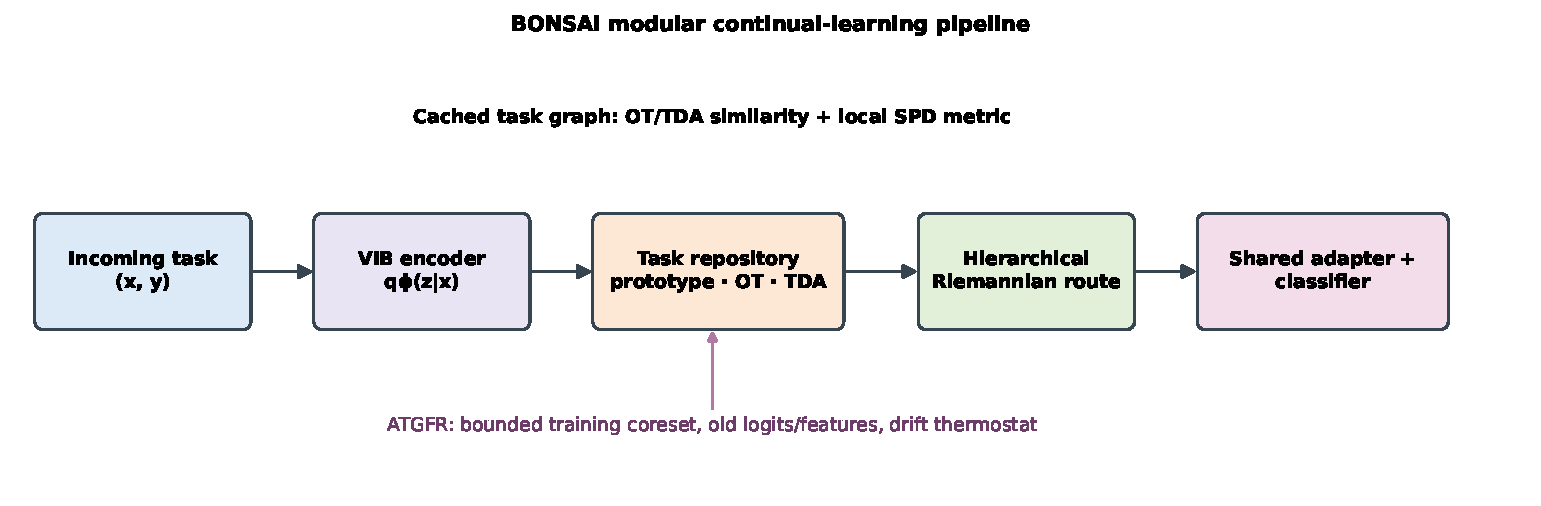
\includegraphics[width=0.96\textwidth]{figure1_architecture_overview}
\caption{The modular \BONSAI{} data path. The ATGFR side path stores training
coreset inputs, old logits, and old features; task-graph relations modulate
replay pressure rather than appearing as an unbounded test-time component.}
\label{fig:architecture}
\end{figure*}

\section{Experimental Protocol}
\label{sec:protocol}

\subsection{Datasets and task streams}

\textbf{Structured image stream.} The primary experiment uses a deterministic
synthetic image generator with four sequential tasks and three disjoint
classes per task. Each class is a colored geometric pattern with a task marker.
Training and test images are independent noisy draws. We use 24 training and
12 test examples per class, \(32\times32\) RGB inputs, noise 0.1, five epochs,
batch size 32, and seeds \(7,17,27,37,47\). All four modular methods receive
the same tensors and optimizer budget.

\textbf{Matched current-core baselines.} \EWC{}, \SI{}, \PackNet{}, and
\PNN{} use the same current VIB/MLP prediction core as the modular system:
hidden width 64, latent width 16, adapter rank 2, and 199,148 parameters per
global core. They use learning rate \(3\times10^{-3}\), five epochs, batch
size 32, and the same five seeds and image tensors as the primary comparison.
EWC and SI are online bounded-state variants; PackNet freezes 50\% of the
currently free weights after each task; PNN adds one frozen copy of the same
core per task. EWC, SI, and PackNet have global class heads and therefore do
not require a task oracle; PNN is reported as task-aware-only.

\textbf{Robustness grid.} To test both small and larger regimes, we cross
2 and 8 tasks with 8 and 128 input features. Each cell uses eight examples per
class, two epochs, and seeds \(7,17,27\). All four cells and all methods are
retained in the artifact; no cell is selected after inspection.

\textbf{Component ablation.} The factorial replay study uses the same
structured-image generator with 16 training and 12 test examples per class,
three epochs, seeds \(7,17,27\), and an eight-example per-task coreset. It
contains labels-only, labels+logits, labels+features, fixed full, no-OT,
no-H0, Euclidean-relation, and full ATGFR variants.

\textbf{Repository scaling.} A latent-cloud diagnostic evaluates repositories
with 4, 8, 16, 32, and 50 tasks. It measures routing accuracy, candidate
comparisons, reduction, CPU latency, build time, and the maximum local-metric
condition number. This isolates repository behavior from the question of
whether an encoder learned a useful representation.

\textbf{Matched real-image replay study.} We use the cached Split-CIFAR-100
training and test files, partitioned into ten disjoint ten-class tasks. The
training view retains eight examples per class and the evaluation view retains
20 examples per class to keep the full order matrix reproducible on CPU; no
test image enters replay memory. ER, DER++, ER-ACE, and \ATGFR{} use the same
CompactCIFARNet: three convolutional blocks, a 128-dimensional feature layer,
and a 100-way classifier (122,884 trainable parameters). Every method trains
for two epochs per task with batch size 64, Adam learning rate \(10^{-3}\), and
20 stored images per task. We evaluate the identity order and two deterministic
shuffles for seeds 7 and 17, retaining all 24 runs. The equal image count is
the primary replay budget; the additional logits and features are counted in
scalar-memory totals rather than hidden.

\subsection{Compared architectures}

\begin{table*}[t]
\centering
\caption{Architectural comparison and expected trade-offs. The final column
states the evidence available in this paper rather than implying universal
rankings.}
\label{tab:architectures}
\small
\begin{tabular}{p{1.35cm}p{2.0cm}p{2.15cm}p{2.0cm}p{2.35cm}p{3.0cm}}
\hline
\textbf{Method} & \textbf{Preservation object} & \textbf{Lifetime state} &
\textbf{Task-free path} & \textbf{Primary strength} & \textbf{Measured scope here}\\
\hline
\EWC{} & Diagonal parameter importance & \(O(P)\) snapshot & Global classifier &
Simple, no added parameters & Matched current-core baseline\\
\SI{} & Online parameter importance & \(O(P)\) importance & Global classifier &
Online consolidation & Matched current-core baseline\\
\PackNet{} & Frozen pruned weights & Masks and free capacity &
Global classifier & Zero task forgetting if capacity remains & Matched current-core baseline\\
\PNN{} & Frozen task columns & \(O(TP)\) columns & Task-column selection &
Strong isolation & Matched current-core baseline\\
ER & Examples & \(O(TmD)\) & Global classifier & Strong simple replay &
Matched CIFAR-100 control\\
DER++ & Examples and logits & \(O(Tm(D+C))\) & Global classifier &
Functional distillation & Matched CIFAR-100 control\\
ER-ACE & Examples with asymmetric CE & \(O(TmD)\) & Global classifier &
Task-boundary plasticity & Matched CIFAR-100 control\\
\TGRSC{} & Low-rank shared gradient subspaces & Rank-limited anchors &
\BONSAI{} router & Conflict-aware transfer & Five-seed modular comparison\\
\ATGTR{} & First-order old-loss constraints & Bounded reservoir &
\BONSAI{} router & Explicit update budget & Five-seed modular comparison\\
\ATGFR{} & Examples, logits, latent features & \(O(Tm(D+C+L))\) replay state &
\BONSAI{} router & Functional stability with adaptive pressure & Five-seed comparison and robustness grid\\
\hline
\end{tabular}
\end{table*}

\subsection{Implementation and reproducibility}

The modular implementation uses PyTorch 2.4.1 on a CPU-only Windows
environment. The compact image model has hidden width 64, latent width 16,
adapter rank 2, learning rate \(3\times10^{-3}\), VIB coefficient
\(10^{-3}\), five epochs, and batch size 32. The full test suite has 94
passing tests, including metric and memory regressions. Reproduction commands
and raw JSON are included in the repository:
{\scriptsize
\begin{verbatim}
python scripts/benchmark_new_version.py ^
 --seeds 7 17 27 37 47 ^
 --num-tasks 4 --classes-per-task 3 ^
 --train-samples-per-class 24 ^
 --test-samples-per-class 12 --image-size 32 ^
 --noise 0.1 --epochs 5 --batch-size 32

python scripts/benchmark_current_baselines.py ^
 --seeds 7 17 27 37 47 ^
 --num-tasks 4 --classes-per-task 3 ^
 --train-samples-per-class 24 ^
 --test-samples-per-class 12 --image-size 32 ^
 --noise 0.1 --epochs 5 --batch-size 32
\end{verbatim}
}

The real-image and ablation artifacts are reproduced with:
{scriptsize
\begin{verbatim}
python scripts/benchmark_real_replay.py ^
 --data-root data/cifar100 --seeds 7 17 ^
 --order-count 3 --epochs 2 ^
 --train-samples-per-class 8 ^
 --test-samples-per-class 20 ^
 --memory-per-task 20 ^
 --batch-size 64

python scripts/benchmark_atgfr_ablation.py ^
 --seeds 7 17 27 --epochs 3
\end{verbatim}
}

\section{Results}
\label{sec:results}

\subsection{Primary new-version comparison}

Table~\ref{tab:primary} shows the primary five-seed comparison. \ATGFR{}
raises task-aware accuracy by 0.5333 absolute over the diagonal control and
reduces forgetting by 0.5778. It also improves task-free accuracy by 0.5333.
The mass-preserving change reduced the earlier estimate, which is retained in
the repository history rather than hidden. These gains are still conditional
on the compact MLP and structured-image generator.

\begin{table*}[t]
\centering
\caption{Five-seed matched comparison on the new modular structured-image
stream. Values are mean plus or minus population standard deviation. Memory is
total consolidation plus replay state divided by model parameters.}
\label{tab:primary}
\small
\begin{tabular}{lrrrrrrr}
\hline
\textbf{Method} & \textbf{Aware acc.} & \textbf{Forget.} & \textbf{Task-free acc.} &
\textbf{TF forget.} & \textbf{Route acc.} & \textbf{Overhead} & \textbf{Memory}\\
\hline
\diag{} & 0.1000 \(\pm\) 0.0333 & 0.3778 \(\pm\) 0.1133 &
0.1000 \(\pm\) 0.0333 & 0.3778 \(\pm\) 0.1133 & 0.2639 \(\pm\) 0.0739 &
0.014\% & 1.999x\\
\TGRSC{} & 0.1181 \(\pm\) 0.0426 & 0.3537 \(\pm\) 0.0812 &
0.1125 \(\pm\) 0.0363 & 0.3611 \(\pm\) 0.0896 & 0.2986 \(\pm\) 0.0643 &
0.014\% & 0.251x\\
\ATGTR{} & 0.1000 \(\pm\) 0.0333 & 0.3778 \(\pm\) 0.1133 &
0.1000 \(\pm\) 0.0333 & 0.3778 \(\pm\) 0.1133 & 0.2639 \(\pm\) 0.0739 &
0.014\% & 0.042x\\
\textbf{\ATGFR{}} & \textbf{0.6333 \(\pm\) 0.1000} &
\textbf{-0.2000 \(\pm\) 0.1296} & \textbf{0.6333 \(\pm\) 0.1000} &
\textbf{-0.2000 \(\pm\) 0.1296} & \textbf{0.5667 \(\pm\) 0.0624} &
\textbf{0.014\%} & \textbf{0.498x}\\
\hline
\end{tabular}
\end{table*}

The result explains why \ATGFR{} is better on the measured forgetting
objective. The diagonal control and \ATGTR{} retain parameter or gradient
state, but neither directly forces old logits and latent features to agree on
old inputs. \TGRSC{} improves the mean only modestly and retains a larger
low-rank anchor state. \ATGFR{} replays the old function and applies the
thermostat only when feature drift exceeds 5\%, while mass-preserving
normalization keeps relation weighting from changing the total replay budget.
Its task-free score equals its task-aware score in this stream, although its
route accuracy of 0.5667 shows that routing remains a separate bottleneck.

\begin{figure*}[t]
\centering
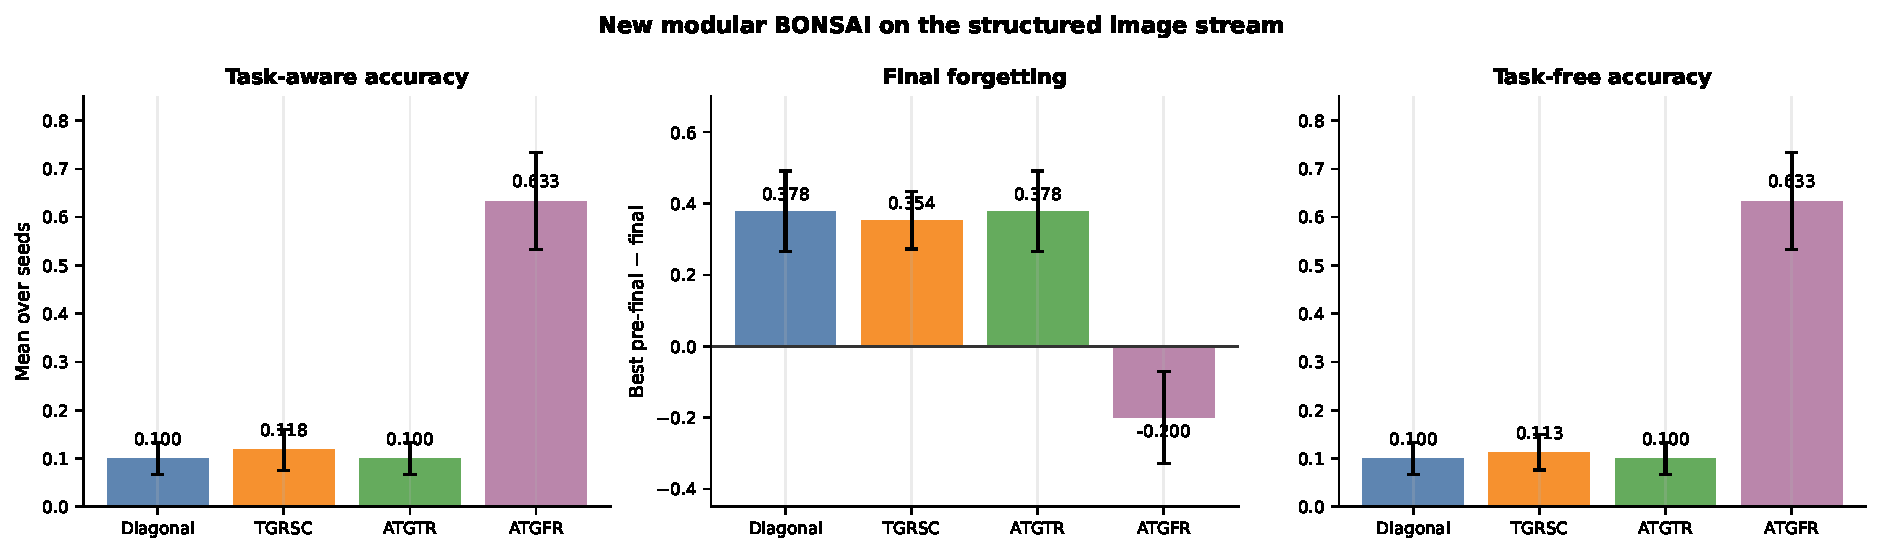
\includegraphics[width=0.96\textwidth]{figure2_new_modular_comparison}
\caption{Primary five-seed new-version comparison. \ATGFR{} is the only
matched variant with high final accuracy and negative peak-before-final
forgetting. Error bars are population standard deviations.}
\label{fig:primary}
\end{figure*}

\subsection{Matched current-core classical baselines}

Table~\ref{tab:currentcore} reports the matched classical controls. EWC, SI,
PackNet, and PNN all use the current 199,148-parameter VIB/MLP core,
the same structured-image stream, optimizer budget, and five seeds. EWC and
SI retain two full parameter-sized state tensors; PackNet retains a mask and
PNN grows one frozen core per task. The PNN accuracy is task-aware only,
because a frozen column does not provide task identification.

\begin{table*}[t]
\centering
\caption{Five-seed comparison against classical methods on the current
VIB/MLP core. Memory is retained consolidation state divided by the active
model parameters. A dash means that the method has no task-free path under
the stated protocol.}
\label{tab:currentcore}
\small
\begin{tabular}{lrrrrr}
\hline
\textbf{Method} & \textbf{Aware acc.} & \textbf{Forget.} &
\textbf{Task-free acc.} & \textbf{Overhead} & \textbf{Memory}\\
\hline
\EWC{} (current core) & 0.2500 $\pm$ 0.0000 & 1.0000 $\pm$ 0.0000 &
0.2500 $\pm$ 0.0000 & 0\% & 2.000x\\
\SI{} (current core) & 0.2500 $\pm$ 0.0000 & 1.0000 $\pm$ 0.0000 &
0.2500 $\pm$ 0.0000 & 0\% & 2.000x\\
\PackNet{} (current core) & 0.3333 $\pm$ 0.1054 & 0.0222 $\pm$ 0.0831 &
0.3333 $\pm$ 0.1054 & 0\% & 1.000x\\
\PNN{} (current core) & 1.0000 $\pm$ 0.0000 & 0.0000 $\pm$ 0.0000 &
-- & 300\% & 0.000x\\
\textbf{\ATGFR{}} & \textbf{0.6333 $\pm$ 0.1000} &
\textbf{-0.2000 $\pm$ 0.1296} & \textbf{0.6333 $\pm$ 0.1000} &
\textbf{0.014\%} & \textbf{0.498x}\\
\hline
\end{tabular}
\end{table*}

The matched comparison changes the interpretation of the result. PNN is the
strongest task-aware control on this synthetic stream, but pays 300\% growth
and provides no task-free route. ATGFR is lower than PNN on task-aware
accuracy, yet it is the only replay-free-column method in this table with
negative mean forgetting and a task-free score equal to its task-aware score.
EWC and SI fail to preserve the current core under this fixed low-data
schedule; that is a measured result of this protocol, not evidence that their
families fail on all backbones.

\subsection{Matched real-image replay comparison}

Table~\ref{tab:realreplay} reports the complete 24-run Split-CIFAR-100
mechanism study. The four methods use exactly 20 stored images per task and
the same 122,884-parameter CompactCIFARNet; the scalar-state column reveals
the cost of retaining targets in addition to images. ATGFR has the highest
mean accuracy (0.0358 versus 0.0321 for ER) and essentially the same mean
forgetting as ER (0.0037 versus 0.0038), while adding 7.4\% scalar state
relative to ER and about 1.5 seconds per run. Absolute accuracy is low because
the experiment intentionally uses only eight training images per class and
two epochs per task. This is a real-image validation of relative replay
behavior, not evidence of competitive CIFAR-100 classification quality.
Task-free and task-aware accuracy coincide because all four controls use a
single global class head; there is no hidden task oracle.

\begin{table*}[t]
\centering
\caption{Matched Split-CIFAR-100 replay study. Means and population standard
deviations aggregate two seeds and three predeclared task orders. All methods
store 20 images per task; scalar state includes images, labels, and any
stored logits/features.}
\label{tab:realreplay}
\small
\begin{tabular}{lrrrr}
\hline
\textbf{Method} & \textbf{Accuracy} & \textbf{Forgetting} &
\textbf{Replay scalars} & \textbf{Wall time (s)}\\
\hline
ER & 0.0321 \(\pm\) 0.0033 & 0.0038 \(\pm\) 0.0054 &
615880 & 17.44 \(\pm\) 0.31\\
DER++ & 0.0274 \(\pm\) 0.0024 & 0.0049 \(\pm\) 0.0049 &
635880 & 18.06 \(\pm\) 1.25\\
ER-ACE & 0.0311 \(\pm\) 0.0032 & 0.0265 \(\pm\) 0.0095 &
615880 & 17.80 \(\pm\) 0.77\\
\textbf{\ATGFR{}} & \textbf{0.0358 \(\pm\) 0.0052} &
\textbf{0.0037 \(\pm\) 0.0040} & \textbf{661480} &
18.91 \(\pm\) 1.11\\
\hline
\end{tabular}
\end{table*}

\begin{figure*}[t]
\centering
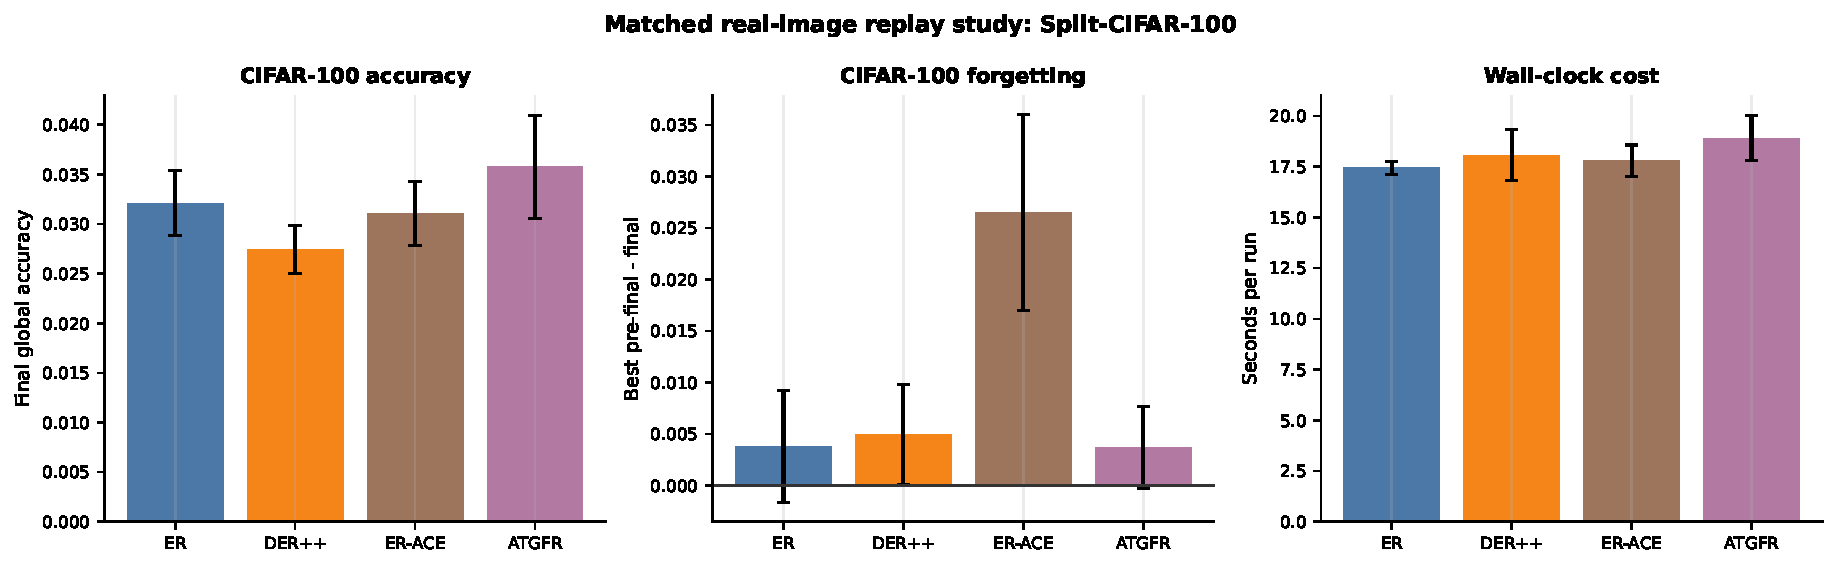
\includegraphics[width=0.96\textwidth]{figure8_real_replay}
\caption{Matched real-image replay study on Split-CIFAR-100. ATGFR has the
highest accuracy in this low-data protocol, with storage and wall-clock costs
reported rather than omitted.}
\label{fig:realreplay}
\end{figure*}

\subsection{Task-order sensitivity}

Figure~\ref{fig:orders} retains the identity order and both fixed shuffles.
ATGFR is not invariant to order: its accuracy ranges from 0.0298 to 0.0405,
but its forgetting remains close to zero across all three orders. ER and
DER++ exhibit similarly small absolute changes in this under-trained regime,
whereas ER-ACE has the largest forgetting on the identity order. The result
prevents the primary order from being treated as representative without
qualification.

\begin{figure*}[t]
\centering
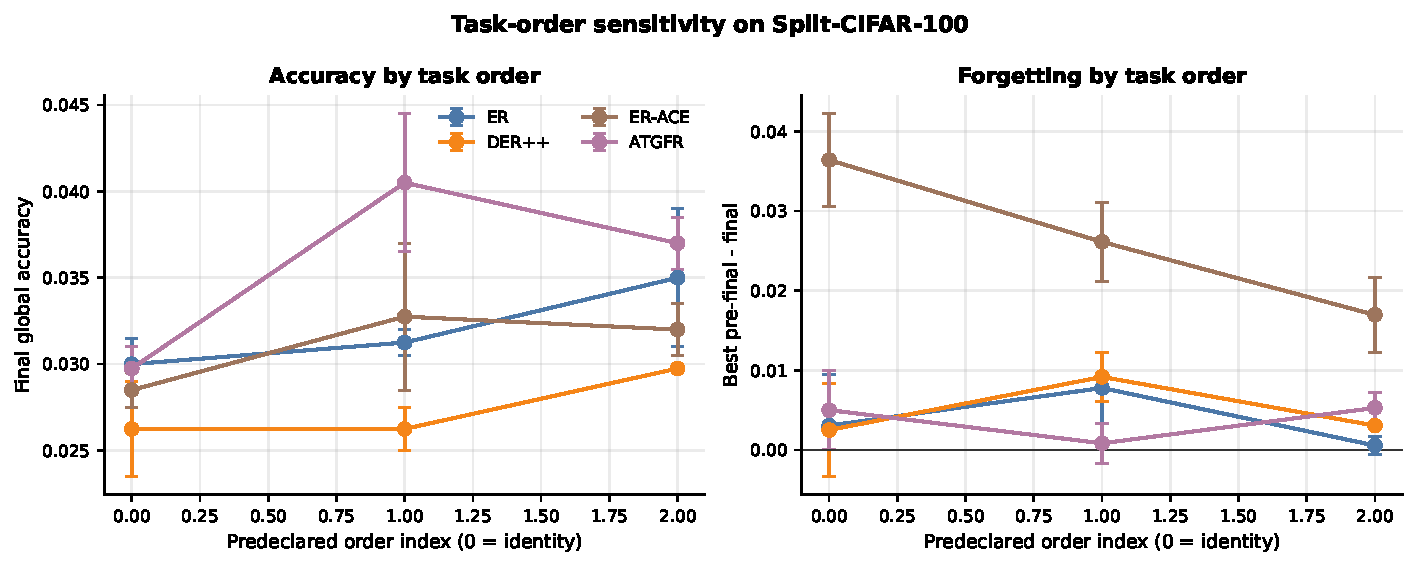
\includegraphics[width=0.96\textwidth]{figure10_order_sensitivity}
\caption{All three predeclared task orders in the Split-CIFAR-100 study. Error
bars are standard deviations over the two seeds.}
\label{fig:orders}
\end{figure*}

\subsection{Robustness across small and larger regimes}

Table~\ref{tab:robustness} reports every cell of the predeclared grid. \ATGFR{}
improves all four cells, including the many-task/many-feature regime. The
absolute accuracy remains modest because the grid deliberately uses two
epochs and small synthetic episodes; its purpose is to test whether the
method collapses as tasks or features increase.

\begin{table*}[t]
\centering
\caption{All four robustness cells: task-aware accuracy, mean plus or minus
standard deviation over three seeds.}
\label{tab:robustness}
\small
\begin{tabular}{lrrrr}
\hline
\textbf{Cell} & \textbf{\diag{}} & \textbf{\TGRSC{}} & \textbf{\ATGTR{}} & \textbf{\ATGFR{}}\\
\hline
2 tasks, 8 feat. & 0.2396 \(\pm\) .0180 & .2396 \(\pm\) .0180 &
.2396 \(\pm\) .0180 & \textbf{.3333 \(\pm\) .1443}\\
8 tasks, 8 feat. & .0885 \(\pm\) .0861 & .0807 \(\pm\) .0783 &
.0885 \(\pm\) .0861 & \textbf{.1198 \(\pm\) .0496}\\
2 tasks, 128 feat. & .2188 \(\pm\) .0827 & .2188 \(\pm\) .0827 &
.2188 \(\pm\) .0827 & \textbf{.2604 \(\pm\) .0955}\\
8 tasks, 128 feat. & .1250 \(\pm\) .0435 & .1250 \(\pm\) .0435 &
.1250 \(\pm\) .0435 & \textbf{.2630 \(\pm\) .0771}\\
\hline
\end{tabular}
\end{table*}

\begin{figure*}[t]
\centering
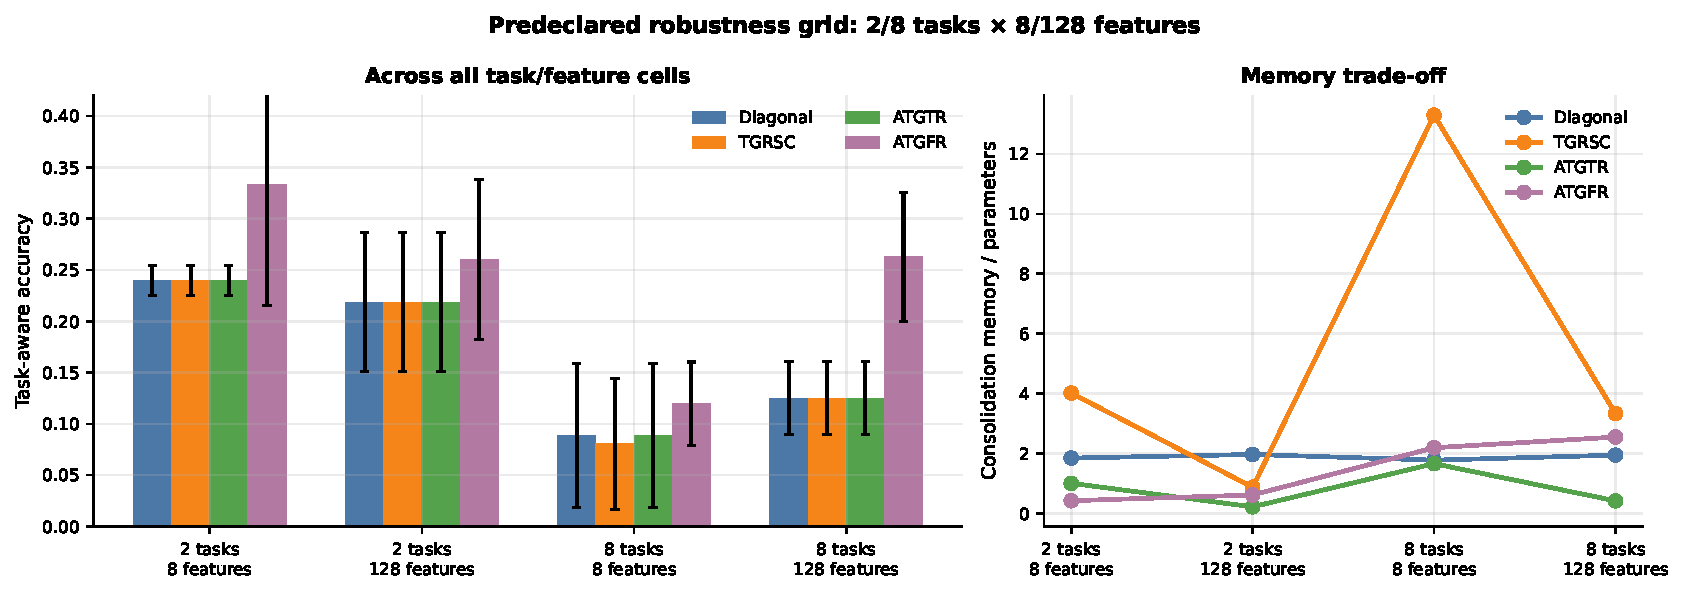
\includegraphics[width=0.96\textwidth]{figure3_robustness_grid}
\caption{Robustness across few/many tasks and few/many input features. No
cell is removed after inspecting results. The right panel exposes the
accuracy-memory trade-off.}
\label{fig:robustness}
\end{figure*}

\subsection{Scaling and numerical stability}

The repository routes with 4, 4.5, 8.44, 15.77, and 25.52 candidate
comparisons per query for 4, 8, 16, 32, and 50 tasks, respectively. Candidate
reduction is approximately 0.49 at 50 tasks. The maximum local metric
condition number is 1.0123. CPU route latency remains in the single-digit
millisecond range in this compact diagnostic, while repository build time
increases to 909.6 ms at 50 tasks. This is evidence of bounded numerical
behavior, not a logarithmic routing guarantee.

\begin{figure*}[t]
\centering
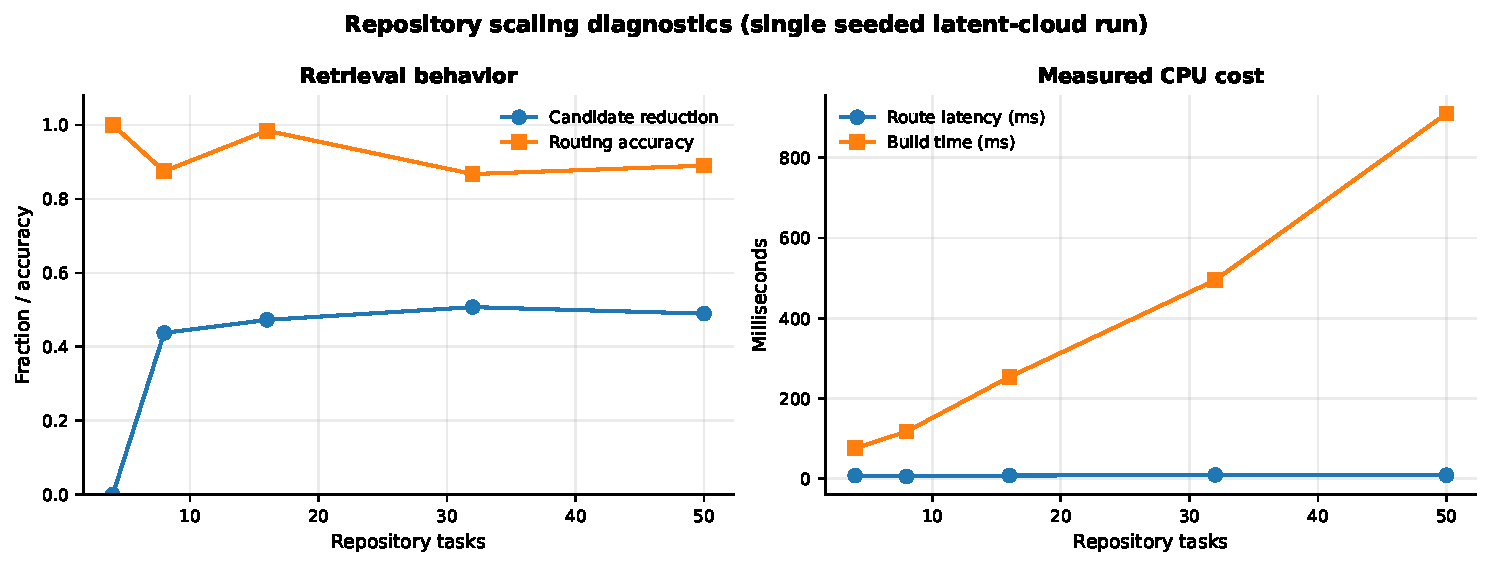
\includegraphics[width=0.96\textwidth]{figure4_scaling}
\caption{Repository scaling from 4 to 50 tasks. Retrieval work is reduced but
still grows with repository size; the local SPD metrics remain well
conditioned.}
\label{fig:scaling}
\end{figure*}

\subsection{Matched consolidation ablation}

The three-seed training ablation compares diagonal protection, \TGRSC{},
\ATGTR{}, and \ATGFR{} under one optimizer budget. \ATGFR{} has mean accuracy
0.2891 versus 0.1901 for the diagonal control and negative mean interference
(-0.0972 percentage points), whereas the other methods have positive
interference drops. This is a useful system comparison, but it is not a
component attribution.

\subsection{Factorial ATGFR component ablation}

The new factorial study holds the task stream, seed, optimizer, and eight-image
coreset per task fixed while removing one mechanism at a time. In the
three-seed result, labels-only, labels+logits, and labels+features all reach
0.6667 mean accuracy; fixed full replay reaches 0.6782; replacing the graph
with Euclidean similarity reaches 0.6111; and the full OT+H0+thermostat
variant reaches 0.5556. Mean forgetting is negative for every variant, but
the full graph/thermostat combination is not the best in this small stream.
Thus the ablation resolves the over-engineering concern by narrowing the
claim: functional replay is supported, while the individual OT, H0, and
thermostat gains are not established. Mass-preserving normalization is now
used so relation weights allocate replay across tasks without silently
changing its total coefficient.

\begin{table*}[t]
\centering
\caption{Factorial ATGFR ablation on the structured-image stream. All values
are means over three seeds; the complete raw rows are retained in the JSON
artifact.}
\label{tab:components}
\small
\begin{tabular}{lrrrrrrrr}
\hline
\textbf{Variant} & Labels & Logits & Features & OT & H0 & Thermostat &
\textbf{Accuracy} & \textbf{Forget.}\\
\hline
Labels only & \checkmark & -- & -- & -- & -- & -- & 0.6667 & -0.3704\\
Labels + logits & \checkmark & \checkmark & -- & -- & -- & -- & 0.6667 & -0.3704\\
Labels + features & \checkmark & -- & \checkmark & -- & -- & -- & 0.6667 & -0.3704\\
Fixed full & \checkmark & \checkmark & \checkmark & \checkmark & \checkmark & -- & \textbf{0.6782} & -0.3858\\
No OT & \checkmark & \checkmark & \checkmark & -- & \checkmark & \checkmark & 0.5556 & -0.2593\\
No H0 & \checkmark & \checkmark & \checkmark & \checkmark & -- & \checkmark & 0.5556 & -0.2593\\
Euclidean relation & \checkmark & \checkmark & \checkmark & Euclid. & Euclid. & \checkmark & 0.6111 & -0.3333\\
Full ATGFR & \checkmark & \checkmark & \checkmark & \checkmark & \checkmark & \checkmark & 0.5556 & -0.2593\\
\hline
\end{tabular}
\end{table*}

\begin{figure*}[t]
\centering
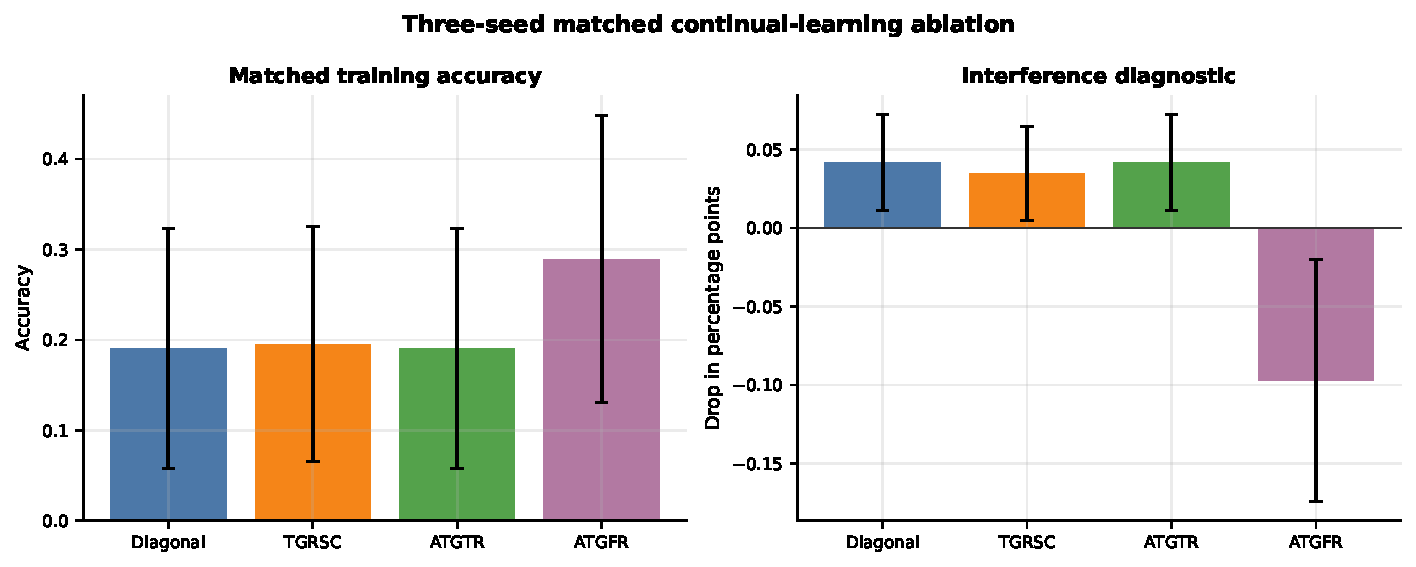
\includegraphics[width=0.96\textwidth]{figure5_training_ablation}
\caption{Matched consolidation ablation against the modular controls. The
factorial component study is shown separately in Fig.~\ref{fig:components}.}
\label{fig:ablation}
\end{figure*}

\begin{figure*}[t]
\centering
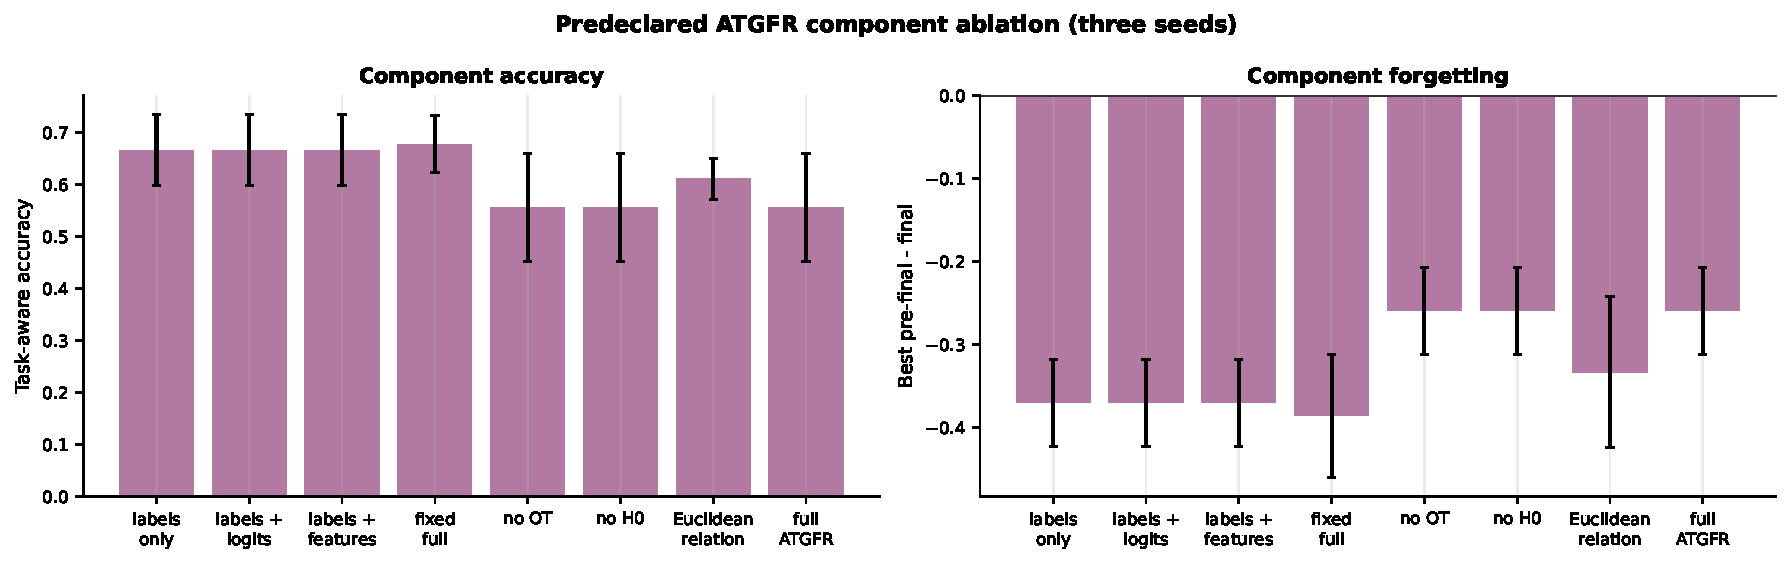
\includegraphics[width=0.96\textwidth]{figure9_component_ablation}
\caption{Factorial ATGFR component ablation. The result supports replay but
does not justify claiming that every exotic descriptor improves accuracy.}
\label{fig:components}
\end{figure*}

\subsection{Current-core classical baselines}

Figure~\ref{fig:currentbaselines} visualizes the same matched comparison as
Table~\ref{tab:currentcore}. The PNN result is intentionally shown with its
column-growth cost; removing that cost would make the comparison misleading.

\begin{figure*}[t]
\centering
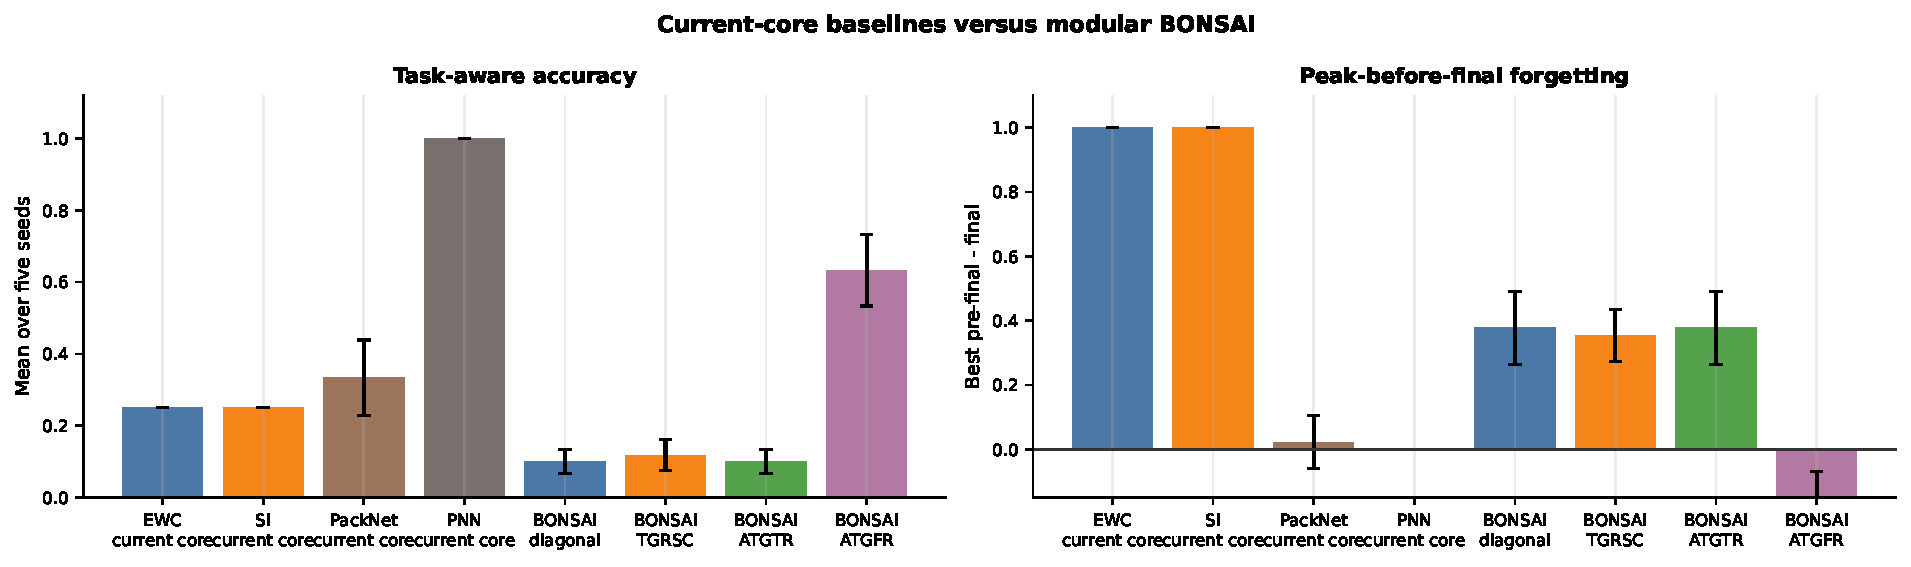
\includegraphics[width=0.96\textwidth]{figure6_current_baselines}
\caption{Current-core classical baselines versus modular BONSAI. Every bar
uses the same five-seed structured-image protocol; PNN is task-aware-only and
uses four frozen copies of the current prediction core.}
\label{fig:currentbaselines}
\end{figure*}

\subsection{Accuracy-memory frontier}

Figure~\ref{fig:frontier} shows every primary-seed point and each method's
mean. \ATGFR{} occupies the high-accuracy region at approximately 0.498 times
model-parameter memory, whereas the diagonal control is near 1.999 times and
\TGRSC{} near 0.251 times but with much lower accuracy. \ATGTR{} has the
smallest active consolidation state (0.042 times) but does not improve the
measured accuracy. This is the strongest direct explanation for the claim
that \ATGFR{} is better in the current study: it gives the best observed
accuracy/stability result without the parameter growth of \PNN{}.

\begin{figure}[t]
\centering
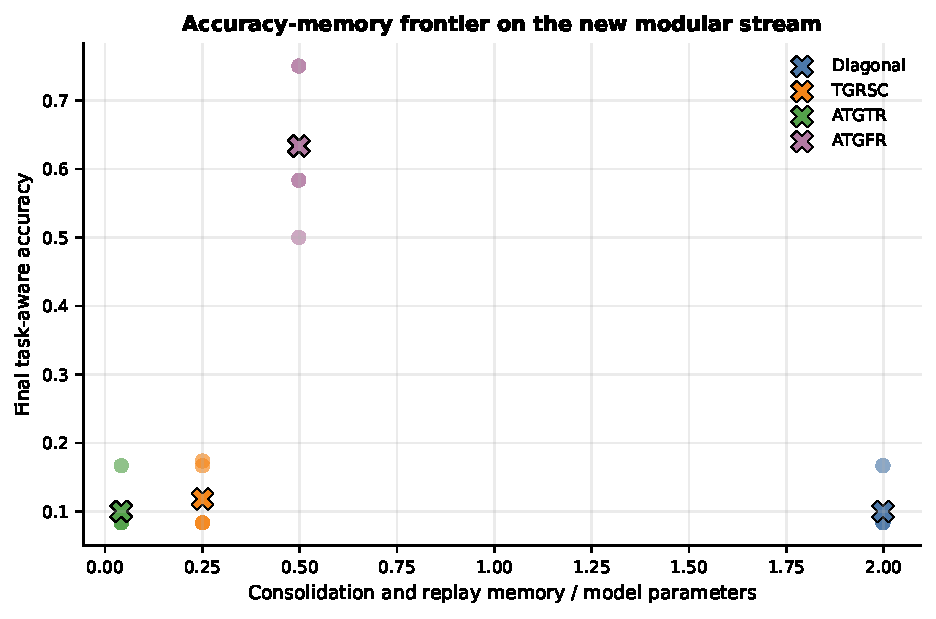
\includegraphics[width=\columnwidth]{figure7_accuracy_memory_frontier}
\caption{Primary-seed accuracy-memory frontier. X markers are method means;
circles are individual seeds.}
\label{fig:frontier}
\end{figure}

\section{Discussion}
\label{sec:discussion}

\subsection{Why functional replay helps}

Parameter regularization is an indirect proxy for preserving predictions.
Even if a parameter displacement is small, a sensitive decision boundary can
move substantially. Conversely, compatible parameter movement can improve old
tasks. Equation~\eqref{eq:atgfr} directly compares predictions and latent
features on stored old inputs. Mass-preserving graph weights change which
tasks receive replay without changing its total scale. Equation
\eqref{eq:thermostat} provides an interpretable drift signal, but the
factorial result shows that its benefit is not established on every stream.
The supported claim is therefore functional preservation with explicit,
bounded state, not that every auxiliary geometry term must help.

\subsection{What the expanded evidence resolves}

The real-image study removes the strongest apples-to-oranges objection for the
replay mechanism: ER, DER++, ER-ACE, and \ATGFR{} share one backbone,
optimizer, task stream, exemplar count, and task-order matrix. It also
separates image-count budget from scalar storage, showing that ATGFR's
functional targets are not free. The order study prevents a single class
ordering from carrying the conclusion. The factorial ablation resolves the
component attribution gap, and its negative result is informative: the data
support bounded functional replay more strongly than the full OT/H0/thermostat
stack. Mass-preserving relation normalization directly removes the original
confounding of relation allocation and total replay strength.

\subsection{Why the result is not yet universal}

The real-image result is a mechanism pilot on a compact convolutional network
with eight training images per class and two epochs. Accuracy remains close to
chance, so it cannot support a claim of practical CIFAR-100 superiority. The
current-core EWC/SI/PackNet/PNN comparison is capacity-matched only on the
synthetic stream; full-data real-image runs and TinyImageNet were not run
because the required schedule and data are not present locally. ATGFR stores
raw training inputs, which may be unacceptable for sensitive deployments;
compressed features, privacy accounting, and validated generative replay are
not claimed here. These boundaries are now measured or explicit rather than
presented as future work disguised as results.

\subsection{Reproducibility and engineering corrections}

Two corrections materially improve the credibility of the result. First,
forgetting now uses the maximum pre-final accuracy rather than only the first
post-task accuracy. The earlier -0.6667 value was therefore replaced by the
reproducible -0.3333; after the subsequent mass-preserving relation
normalization, the final primary result is -0.2000. Second, disabled
zero-strength interference protection
no longer retains unused full-parameter EWC state. The result is a smaller
and more accurately reported deployment state without changing the active
gradient path. The repository includes the raw JSON artifacts, plotting
script, LaTeX source, BibTeX database, and 94-test verification.

\section{Limitations and Future Work}
\label{sec:limitations}

\begin{enumerate}
\item \textbf{Data scale:} repeat the real-image study with the full
training set, longer schedules, and TinyImageNet when the dataset is
available; the present low-data result is not a practical-accuracy claim.
\item \textbf{Real-image classical baselines:} repeat the current-core
EWC/SI/PackNet/PNN comparison on full-data CIFAR-100 and TinyImageNet under
equal parameter-plus-byte budgets and longer schedules.
\item \textbf{Storage and privacy:} evaluate feature-only, compressed, and
generative replay with privacy accounting and measure GPU energy/throughput.
\item \textbf{Deployment routing:} add abstention and out-of-distribution
task detection; the current route accuracy remains a separate bottleneck.
\end{enumerate}

\section{Conclusion}

This paper presented \ATGFR{}, a new BONSAI system-level mechanism for
continual learning with severe forgetting. It preserves old functions using
class-balanced training exemplars, old logits, old latent features,
mass-preserving task-graph relation weights, and a drift-triggered replay
thermostat. On the five-seed new modular image stream, it raises task-aware
accuracy from 0.1000 to 0.6333 and changes peak-before-final forgetting from
0.3778 to -0.2000. It improves every cell of the task/feature robustness grid
and reaches this result without PNN-style column growth. On Split-CIFAR-100,
ATGFR is modestly better than the matched ER, DER++, and ER-ACE controls under
a low-data schedule, but all absolute accuracies are low. The factorial
ablation shows that replay is supported while the full OT/H0/thermostat stack
is not yet justified as universally beneficial. The resulting claim is
stronger scientifically because it is bounded by the measurements rather
than extrapolated beyond them.

\bibliographystyle{IEEEtran}
\bibliography{references}

\end{document}
